\documentclass[conference]{IEEEtran}
\IEEEoverridecommandlockouts
\usepackage[T1]{fontenc}
\usepackage{cite}
\usepackage{amsmath,amssymb,amsfonts}
\usepackage{graphicx}
\usepackage{textcomp}
\usepackage{booktabs}
\usepackage{array}
\usepackage{tikz}
\usetikzlibrary{arrows.meta,positioning,shapes.geometric}

\def\BibTeX{{\rm B\kern-.05em{\sc i\kern-.025em b}\kern-.08em
    T\kern-.1667em\lower.7ex\hbox{E}\kern-.125emX}}

\begin{document}

\title{Design and Comparative Evaluation of a 2-Way Set-Associative Cache with LRU Replacement Against a Direct-Mapped Baseline}

\author{
\IEEEauthorblockN{1\textsuperscript{st} Punit}
\IEEEauthorblockA{\textit{Dept. of Computer Science and Engineering} \\
\textit{Rishihood University}\\
Sonipat, India \\
punit.2024@nst.rishihood.edu.in}
\and
\IEEEauthorblockN{2\textsuperscript{nd} Yash Kumar}
\IEEEauthorblockA{\textit{Dept. of Computer Science and Engineering} \\
\textit{Rishihood University}\\
Sonipat, India \\
yash.kumar2024@nst.rishihood.edu.in}
\and
\IEEEauthorblockN{3\textsuperscript{rd} Dhruv Kumar}
\IEEEauthorblockA{\textit{Dept. of Computer Science and Engineering} \\
\textit{Rishihood University}\\
Sonipat, India \\
dhruv.kumar2024@nst.rishihood.edu.in}
\and
\IEEEauthorblockN{4\textsuperscript{th} Ritesh}
\IEEEauthorblockA{\textit{Dept. of Computer Science and Engineering} \\
\textit{Rishihood University}\\
Sonipat, India \\
ritesh.2024@nst.rishihood.edu.in}
\and
\IEEEauthorblockN{5\textsuperscript{th} Parul}
\IEEEauthorblockA{\textit{Dept. of Computer Science and Engineering} \\
\textit{Rishihood University}\\
Sonipat, India \\
parul.2024@nst.rishihood.edu.in}
}

\maketitle

\begin{abstract}
Cache organization is a first-order driver of memory-system performance, yet the cost/benefit trade-off of adding associativity is rarely made concrete for students designing cache hardware from scratch. This paper presents the Phase~I design of two competing cache architectures implemented in Verilog for a Modern Computer Architecture course project: a direct-mapped cache and a 2-way set-associative cache with least-recently-used (LRU) replacement, both sized to hold an identical 2~KB of data so that any difference in behavior is attributable to associativity alone rather than capacity. We detail the address decomposition, module-level architecture, and finite-state-machine control logic shared by both designs, and describe the trace-driven evaluation methodology -- randomized, locality-biased, and adversarial conflict-access traces -- used to measure hit rate, together with the FPGA synthesis flow used to quantify the resource and timing cost of the second way. Both designs are implemented and verified in simulation: on the conflict trace the direct-mapped cache hits on 0.00\% of accesses while the 2-way cache hits on 99.90\%, and on the locality trace the 2-way cache raises the hit rate from 88.35\% to 89.40\% and cuts average access time from 3.06 to 1.90 cycles. FPGA resource and timing results will be reported in the project's next phase once synthesis is finalized.
\end{abstract}

\begin{IEEEkeywords}
cache memory, set-associative cache, direct-mapped cache, LRU replacement, FPGA, Verilog, computer architecture
\end{IEEEkeywords}

\section{Introduction}
The gap between processor and main-memory speed makes the cache the single most influential structure in a memory hierarchy's observed performance~\cite{hennessy2017}. A cache's \emph{placement policy} -- how many possible locations a given memory block may occupy -- determines how it behaves when two unrelated addresses compete for the same storage. A direct-mapped cache, which permits exactly one location per block, is simple and fast to access but is uniquely vulnerable to \emph{conflict misses}: two addresses that alias to the same index evict one another even when the rest of the cache is empty. Increasing associativity gives each address more than one possible home, trading additional comparison and replacement-selection hardware for a lower miss rate. This project implements and compares the two simplest points on that spectrum -- one-way (direct-mapped) and two-way set-associative with LRU replacement -- as a hands-on vehicle for quantifying that trade-off in actual synthesizable RTL rather than in simulation alone.

\section{Literature Review}
The placement and replacement problem this project investigates has been studied since the earliest cache designs. Smith's 1982 survey of cache memories remains the standard reference for the design space explored here: it catalogs fetch, placement, and replacement policies and establishes that replacement-policy choice matters only once a cache is set-associative or fully associative, since a direct-mapped cache has no replacement decision to make at all~\cite{smith1982}. The same survey documents the earliest trace-driven simulation methodology for measuring miss rate as a function of associativity, which this project adopts in simplified form through its three synthetic access traces.

Hennessy and Patterson's \emph{Computer Architecture: A Quantitative Approach} formalizes the three-way classification of cache misses -- compulsory, capacity, and conflict -- and shows empirically that, across cache sizes from 4~KB to 512~KB, the largest reduction in miss rate comes from moving from direct-mapped to two-way associativity, with diminishing returns at four-way and eight-way~\cite{hennessy2017}. This result is the direct motivation for this project's choice of comparison: two-way associativity is where the per-access hardware cost of associativity (an extra tag comparator and a replacement bit per set) first has to be weighed against a miss-rate reduction large enough to matter, which is exactly the trade-off Section~III and the project's forthcoming results quantify. The undergraduate treatment in Patterson and Hennessy's \emph{Computer Organization and Design} supplies the address-decomposition and tag/index/offset formalism this project's RTL follows directly~\cite{patterson2011}.

Beyond plain LRU, a substantial body of later work shows that recency alone is an imperfect predictor of reuse, particularly for workloads whose working set exceeds the cache or that scan over data with no temporal locality. Qureshi et al.\ introduced the LRU Insertion Policy and Bimodal Insertion Policy, which change \emph{where} an incoming line is inserted in the recency order rather than changing the recency tracking itself, specifically to prevent LRU from thrashing on memory-intensive workloads~\cite{qureshi2007}. Jaleel et al.\ generalized this idea into Re-Reference Interval Prediction (RRIP), a 2-bit-per-line scheme that predicts \emph{when} a line will next be used instead of only tracking how recently it was used, and showed it outperforms LRU and its insertion-policy variants across SPEC CPU2006 and multimedia workloads on a last-level cache~\cite{jaleel2010}. These results motivate plain LRU as the correct replacement policy for a first, two-way design -- it is the mechanism every more sophisticated policy in this line of work is explicitly built to improve upon -- while identifying adaptive or re-reference-based replacement as the natural next direction once this project's two-way/LRU baseline is characterized.

\section{Proposed Solution}
\subsection{Design Parameters}
Both caches are sized to hold an identical 2~KB of data over a 32-bit byte address, so that the comparison in the project's results isolates the effect of associativity rather than capacity. Table~\ref{tab:params} gives the address decomposition used by the RTL for each design.

\begin{table}[h]
\centering
\caption{Design Parameters (Matched 2~KB Capacity)}
\label{tab:params}
\begin{tabular}{@{}lcc@{}}
\toprule
\textbf{Parameter} & \textbf{Direct-mapped} & \textbf{2-way set-assoc.} \\
\midrule
Address width & 32 bit & 32 bit \\
Block size & 16 B (4 words) & 16 B (4 words) \\
Lines / sets & 128 lines & 64 sets $\times$ 2 ways \\
Offset bits & 4 & 4 \\
Index bits & 7 & 6 \\
Tag bits & 21 & 22 \\
Replacement & n/a & LRU, 1 bit/set \\
\bottomrule
\end{tabular}
\end{table}

\subsection{Architecture}
Fig.~\ref{fig:arch} shows the shared architecture of the 2-way design. A single controller finite-state machine (FSM) is wired to four parallel state blocks -- the two ways' data/tag RAMs, the tag comparator, and the combined valid/LRU state -- and is the only block that talks to main memory, driving the memory-side request and handshake signals directly. The direct-mapped baseline uses the same controller skeleton, with identical CPU-side and memory-side ports, and the two-way-specific blocks (the second way and the LRU state) removed, which keeps the two designs' external interfaces identical and lets both be driven by the same testbench and trace files.

\begin{figure}[h]
\centering
\resizebox{\columnwidth}{!}{%
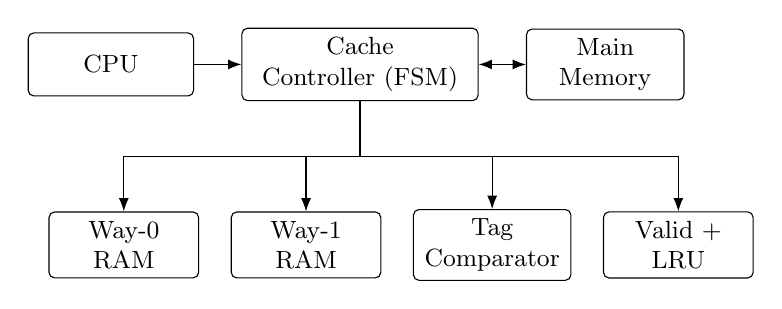
\begin{tikzpicture}[
  box/.style={draw, rounded corners=2pt, minimum width=2.1cm, minimum height=0.8cm, align=center, font=\small},
  node distance=6mm and 6mm
]
\node[box] (cpu) {CPU};
\node[box, right=of cpu, minimum width=3.0cm] (ctrl) {Cache\\Controller (FSM)};
\node[box, right=of ctrl, minimum width=2.0cm] (mm) {Main\\Memory};

\node[box, below=14mm of ctrl, xshift=-3.0cm, minimum width=1.9cm] (w0) {Way-0\\RAM};
\node[box, right=4mm of w0, minimum width=1.9cm] (w1) {Way-1\\RAM};
\node[box, right=4mm of w1, minimum width=2.0cm] (cmp) {Tag\\Comparator};
\node[box, right=4mm of cmp, minimum width=1.9cm] (lru) {Valid +\\LRU};

\draw[-{Latex}] (cpu) -- (ctrl);
\draw[{Latex}-{Latex}] (ctrl) -- (mm);

\draw (ctrl.south) -- ++(0,-7mm) coordinate (bus);
\draw (w0.north |- bus) -- (lru.north |- bus);
\foreach \n in {w0,w1,cmp,lru} \draw[-{Latex}] (\n.north |- bus) -- (\n.north);
\end{tikzpicture}%
}
\caption{One controller FSM coordinates both ways, the tag comparator, and valid/LRU state on every access; only the controller talks to main memory.}
\label{fig:arch}
\end{figure}

\subsection{Control Logic}
Table~\ref{tab:fsm} gives the controller's state transition table for the 2-way design. The direct-mapped baseline uses the same six-state skeleton (\textsc{Idle}, \textsc{Tag\_Check}, \textsc{Hit}, \textsc{Write\_Back}, \textsc{Fetch\_Block}, \textsc{Fill\_Line}) without a victim-selection step, since it has only one possible line per index.

\begin{table}[h]
\centering
\caption{2-Way Cache Controller State Transitions}
\label{tab:fsm}
\begin{tabular}{@{}p{2.15cm}p{5.9cm}@{}}
\toprule
\textbf{State} & \textbf{Action / next state} \\
\midrule
\textsc{Idle} & On a CPU request, latch the address; go to \textsc{Tag\_Check}. \\
\textsc{Tag\_Check} & Compare the incoming tag against both ways' tags in parallel. Hit $\Rightarrow$ \textsc{Hit}; miss $\Rightarrow$ \textsc{Select\_Victim}. \\
\textsc{Hit} & Read or update the hit way; mark it most-recently-used; return to \textsc{Idle}. \\
\textsc{Select\_Victim} & Read the LRU bit for this set to choose the victim way. Dirty victim $\Rightarrow$ \textsc{Write\_Back}; else $\Rightarrow$ \textsc{Fetch\_Block}. \\
\textsc{Write\_Back} & Write the victim's dirty line to memory; on completion $\Rightarrow$ \textsc{Fetch\_Block}. \\
\textsc{Fetch\_Block} & Request the missing block from memory; on completion $\Rightarrow$ \textsc{Fill\_Way}. \\
\textsc{Fill\_Way} & Write data/tag/valid for the victim way; mark it most-recently-used; retry $\Rightarrow$ \textsc{Tag\_Check}. \\
\bottomrule
\end{tabular}
\end{table}

\subsection{Evaluation Methodology}
Both caches expose an identical CPU-side and memory-side interface, so a single trace-driven testbench can drive either one. Three synthetic access traces are used: (i) a uniformly random trace, which exercises ordinary compulsory/capacity behavior; (ii) a locality-biased trace, where 90\% of accesses fall within a small working set, modeling typical program behavior; and (iii) an adversarial conflict trace, in which two addresses are chosen to alias to the same direct-mapped index while differing in tag, which the direct-mapped cache cannot hold simultaneously but the 2-way cache can. Hit rate and average access latency are measured for both caches on all three traces, and both designs are synthesized for the same FPGA target so that look-up-table, flip-flop, and block-RAM utilization and maximum clock frequency can be reported alongside the hit-rate numbers -- giving a joint area/performance comparison rather than a hit-rate number in isolation. Synthesis results are being finalized and will be reported in the project's next phase.

\subsection{Prototype Status and Verification Results}
The RTL for both caches is complete and passes 63 automated checks: unit tests of every submodule, the memory model at three latencies, smoke tests of each cache, a dirty-line write-back test, and a head-to-head conflict test. In that conflict test both caches read addresses \texttt{0x000} and \texttt{0x800} alternately; both map to direct-mapped line~0 and to 2-way set~0. The direct-mapped cache misses on all five accesses, while the 2-way cache misses only on the two cold fills and then hits, because the two blocks occupy different ways of the same set.

Table~\ref{tab:results} gives the trace-driven results over 2,000 accesses per trace. A golden reference model checks every read, and neither cache returns a single incorrect word. The conflict trace shows the effect associativity is meant to remove; on the random trace, whose 64~KB address range is far larger than the 2~KB cache, both caches hit about 3\% of the time and the small difference is noise.

\begin{table}[h]
\centering
\caption{Trace-Driven Simulation Results (2,000 Accesses per Trace)}
\label{tab:results}
\begin{tabular}{@{}lcccc@{}}
\toprule
 & \multicolumn{2}{c}{\textbf{Hit rate}} & \multicolumn{2}{c}{\textbf{Avg.\ cycles/access}} \\
\cmidrule(lr){2-3}\cmidrule(l){4-5}
\textbf{Trace} & \textbf{DM} & \textbf{2-way} & \textbf{DM} & \textbf{2-way} \\
\midrule
Random   & 3.35\%  & 3.00\%  & 10.83 & 9.69 \\
Locality & 88.35\% & 89.40\% & 3.06  & 1.90 \\
Conflict & 0.00\%  & 99.90\% & 10.00 & 1.01 \\
\bottomrule
\end{tabular}
\end{table}

\section{Individual Contributions}
\textbf{Punit} implemented the direct-mapped baseline cache controller and its verification testbench, authored the cache design-parameter specification, and wrote the Proposed Solution section of this report.

\textbf{Yash Kumar} implemented the Way-0/Way-1 data and tag RAM modules and the behavioral main-memory model, and set up the project repository, build instructions, and version control.

\textbf{Dhruv Kumar} implemented the valid-bit, LRU-state, and tag-comparator modules, and conducted the literature review in this report.

\textbf{Ritesh} implemented the 2-way cache controller finite-state machine and the top-level integration of all submodules, and is directing the project's prototype demonstration video.

\textbf{Parul} developed the trace-generation and comparison-testbench methodology described in Section~III-D, will run FPGA synthesis and the hit-rate/resource analysis in the project's next phase, and wrote the Abstract and compiled the references for this report.

\begin{thebibliography}{00}
\bibitem{hennessy2017} J. L. Hennessy and D. A. Patterson, \emph{Computer Architecture: A Quantitative Approach}, 6th ed. Cambridge, MA, USA: Morgan Kaufmann, 2017.
\bibitem{patterson2011} D. A. Patterson and J. L. Hennessy, \emph{Computer Organization and Design: The Hardware/Software Interface}, 4th ed. Waltham, MA, USA: Morgan Kaufmann, 2011.
\bibitem{smith1982} A. J. Smith, ``Cache memories,'' \emph{ACM Comput. Surv.}, vol. 14, no. 3, pp. 473--530, Sep. 1982.
\bibitem{jaleel2010} A. Jaleel, K. B. Theobald, S. C. Steely Jr., and J. Emer, ``High performance cache replacement using re-reference interval prediction (RRIP),'' in \emph{Proc. 37th Int. Symp. Comput. Archit. (ISCA)}, Saint-Malo, France, Jun. 2010, pp. 60--71.
\bibitem{qureshi2007} M. K. Qureshi, A. Jaleel, Y. N. Patt, S. C. Steely Jr., and J. Emer, ``Adaptive insertion policies for high-performance caching,'' in \emph{Proc. 34th Int. Symp. Comput. Archit. (ISCA)}, San Diego, CA, USA, Jun. 2007, pp. 381--391.
\end{thebibliography}

\end{document}